% answers.tex —— 1977 年·吉林卷 · 参考答案与详细解析片段
% 由 tools/generate_projects.py 依来源总账自 1977/1977_数学真题_吉林_试题.md + 1977/1977_数学真题_吉林_解析正文.md + 1977/1977_数学真题_吉林_答案要点.md 生成，勿手改（改源 MD 后重跑）


\begin{gktip}
固定源《吉林1977年高考数学试题解》是题面与解答连排的扫描材料（书籍页码 20—24）。下文逐题对照源解答并重新计算关键结论：第一、四两大题的小题与第二大题的小问印作「1．、2．……」，已按本库小问连续编号规范重排为（1）（2）……；源卷排印用字「园」在解析中按现代用字写作「圆」；第 4 题（2）源卷真数大写 $C$ 的记号问题见题面源注，推导按小写 $c$ 处理；第 4 题（3）源卷函数记号 Sin、Cos、tg 在推导中按 sin、cos、tan 处理，结论一致。
\end{gktip}

\begin{answer}
\gksolhead{1}{}

\textbf{题目}：

（1） 什么是因式分解？把 $18a^3-48a^2b+32ab^2$ 分解因式。

\Needspace{5\baselineskip}
（2） 什么是方程？什么是方程的解？解方程：

\nopagebreak[4]
\[
\frac{2}{x-2}+x=\frac{x}{x-2}.
\]

（3） 在 $\triangle ABC$ 中，$\angle C$ 是直角，$CD$ 是 $AB$ 上的高，已知 $AB=9$，$AC=6$，求 $CD$。

\begin{gktip}
原源 PDF 第 2 页附有直角三角形与斜边上的高 $CD$ 的示意图；LaTeX 版按源图重绘。
\end{gktip}
\nopagebreak[4]
\begin{center}% 1977 年吉林卷第 1 题（3）：直角三角形 ABC，∠C 为直角（带直角标记），
% CD 为斜边 AB 上的高，D 在 AB 上（按源卷第 2 页布局：B 在上、C 左下、A 右下）
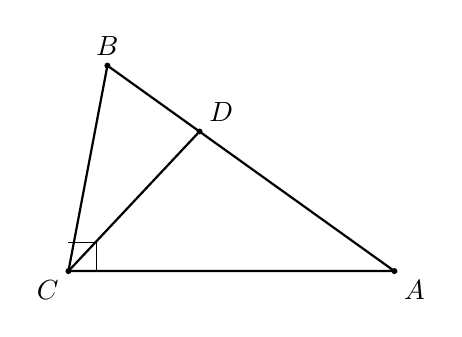
\begin{tikzpicture}[scale=0.9]
  \coordinate (C) at (0,0);
  \coordinate (A) at (4.6,0);
  \coordinate (B) at (0.55,2.9);
  \coordinate (D) at (1.85,1.97);
  \draw[thick] (A)--(B)--(C)--cycle;
  \draw[thick] (C)--(D);
  \draw (0.4,0) -- (0.4,0.4) -- (0,0.4);
  \fill (A) circle (1.2pt) node[below right] {$A$};
  \fill (B) circle (1.2pt) node[above] {$B$};
  \fill (C) circle (1.2pt) node[below left] {$C$};
  \fill (D) circle (1.2pt) node[above right] {$D$};
\end{tikzpicture}
\end{center}
\nopagebreak[4]
\Needspace{4\baselineskip}
\textbf{解析}

\gksubpart{（1）}

\Needspace{5\baselineskip}
把一个多项式分解成几个整式连乘（积）的形式，叫做多项式的因式分解。对原式先提出公因式 $2a$，再用平方差公式的逆用把括号内的二次式写成两数差的平方：

\nopagebreak[4]
\[
18a^3-48a^2b+32ab^2
=2a(9a^2-24ab+16b^2)
=2a(3a-4b)^2.
\]

\gksubpart{（2）}

含有未知数的等式叫做方程；使方程两端相等的未知数的值叫做方程的解。

\Needspace{5\baselineskip}
原方程有分母 $x-2$，须 $x\ne2$。去分母，两端同乘 $x-2$：

\nopagebreak[4]
\[
2+x(x-2)=x.
\]

\Needspace{5\baselineskip}
整理得

\nopagebreak[4]
\[
x^2-3x+2=0,
\qquad
(x-2)(x-1)=0,
\]

所以 $x_1=2$，$x_2=1$。把 $x=2$ 代入原方程，分母为零，故 $x=2$ 是增根，舍去。原方程的解是 $x=1$。

\gksubpart{（3）}

\Needspace{5\baselineskip}
因为 $\angle C$ 是直角，$\triangle ABC$ 是直角三角形。由勾股定理，

\nopagebreak[4]
\[
BC=\sqrt{AB^2-AC^2}
=\sqrt{81-36}=3\sqrt5.
\]

\Needspace{5\baselineskip}
又 $CD$ 是斜边 $AB$ 上的高，用面积关系

\nopagebreak[4]
\[
\frac12\,AB\cdot CD=\frac12\,AC\cdot BC,
\]

\Needspace{5\baselineskip}
得

\nopagebreak[4]
\[
CD=\frac{AC\cdot BC}{AB}
=\frac{6\cdot3\sqrt5}{9}
=2\sqrt5.
\]
\nopagebreak[4]
\begin{center}% 1977 年吉林卷第 1 题（3）：直角三角形 ABC，∠C 为直角（带直角标记），
% CD 为斜边 AB 上的高，D 在 AB 上（按源卷第 2 页布局：B 在上、C 左下、A 右下）
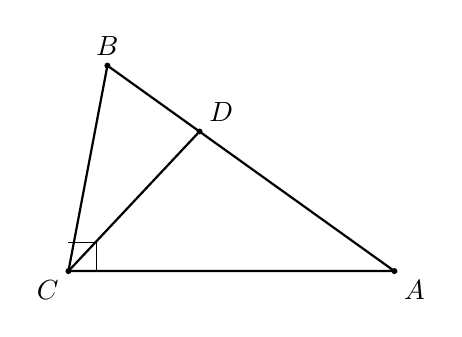
\begin{tikzpicture}[scale=0.9]
  \coordinate (C) at (0,0);
  \coordinate (A) at (4.6,0);
  \coordinate (B) at (0.55,2.9);
  \coordinate (D) at (1.85,1.97);
  \draw[thick] (A)--(B)--(C)--cycle;
  \draw[thick] (C)--(D);
  \draw (0.4,0) -- (0.4,0.4) -- (0,0.4);
  \fill (A) circle (1.2pt) node[below right] {$A$};
  \fill (B) circle (1.2pt) node[above] {$B$};
  \fill (C) circle (1.2pt) node[below left] {$C$};
  \fill (D) circle (1.2pt) node[above right] {$D$};
\end{tikzpicture}
\end{center}
\nopagebreak[4]
\gkanswer{答案（1）：把一个多项式分解成几个整式连乘（积）的形式叫做因式分解；$18a^3-48a^2b+32ab^2=2a(3a-4b)^2$。}

\gkanswer{答案（2）：含有未知数的等式叫做方程，使方程两端相等的未知数的值叫做方程的解；原方程的解为 $x=1$（$x=2$ 是增根，舍去）。}

\gkanswer{答案（3）：$CD=2\sqrt5$。}

\end{answer}
\begin{answer}
\gksolhead{2}{}

\textbf{题目}：

$k$ 是什么值时，方程 $x^2+4x+k=0$ 有

（1） 两个不相等的实根？

（2） 相等的实根？

（3） 没有实根？

\Needspace{4\baselineskip}
\textbf{解析}

\Needspace{5\baselineskip}
方程 $x^2+4x+k=0$ 的判别式为

\nopagebreak[4]
\[
\Delta=4^2-4k=4(4-k).
\]

\gksubpart{（1）}

$k<4$ 时 $\Delta>0$，方程有两个不相等的实根。

\gksubpart{（2）}

$k=4$ 时 $\Delta=0$，方程有两个相等的实根。

\gksubpart{（3）}

$k>4$ 时 $\Delta<0$，方程没有实根。

\gkanswer{答案（1）：$k<4$。}

\gkanswer{答案（2）：$k=4$。}

\gkanswer{答案（3）：$k>4$。}

\end{answer}
\begin{answer}
\gksolhead{3}{}

\textbf{题目}：

什么是平面上的轨迹？

某港口外海面上，有一个暗礁区，为进港船只的安全，建有 $A\text{、}B$ 两灯塔，把暗礁区所张的危险的角 $\angle AMB$ 的大小通知船上。试用轨迹涵义证明：只要进港船只 $S$ 的视角 $\angle ASB<\angle AMB$ 时，船只就可安全进港。

\begin{gktip}
原源 PDF 第 2 页附有灯塔 $A\text{、}B$、圆弧上的点 $M$ 与船只 $S$ 的示意图；LaTeX 版按源图重绘。
\end{gktip}
\nopagebreak[4]
\begin{center}% 1977 年吉林卷第 3 题：港口暗礁轨迹示意——圆内弦 AB、圆周角顶点 M（在圆上）
% 与圆外船只 S，S、M、B 共线，另画 SA 与 AM（按源卷第 2 页布局：S 在上、AB 在下）
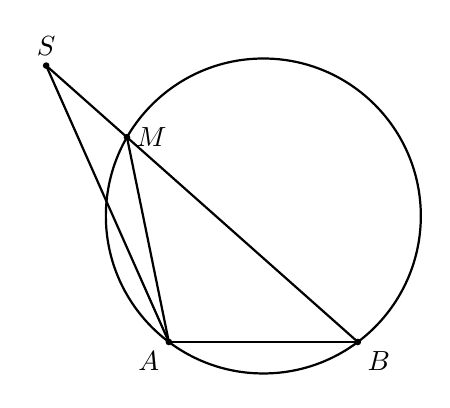
\begin{tikzpicture}[scale=1.0]
  \draw[thick] (0,0) circle (2);
  \coordinate (A) at (-1.2,-1.6);
  \coordinate (B) at (1.2,-1.6);
  \coordinate (M) at (-1.732,1);
  \coordinate (S) at (-2.758,1.91);
  \draw[thick] (S)--(B);
  \draw[thick] (S)--(A);
  \draw[thick] (A)--(B);
  \draw[thick] (A)--(M);
  \fill (A) circle (1.2pt) node[below left] {$A$};
  \fill (B) circle (1.2pt) node[below right] {$B$};
  \fill (M) circle (1.2pt) node[right] {$M$};
  \fill (S) circle (1.2pt) node[above] {$S$};
\end{tikzpicture}
\end{center}
\nopagebreak[4]
\Needspace{4\baselineskip}
\textbf{解析}

平面上的动点按照一定规律运动所描绘的图形，就叫做动点在平面上的轨迹。

两灯塔 $A\text{、}B$ 之间的距离为定长，暗礁区所张的角 $\angle AMB$ 为定角，因此顶点 $M$ 的轨迹是以 $AB$ 为弦、对弦 $AB$ 张角等于定角 $\angle AMB$ 的圆弧，暗礁区就在这段圆弧的内侧：
\nopagebreak[4]
\begin{center}% 1977 年吉林卷第 3 题：港口暗礁轨迹示意——圆内弦 AB、圆周角顶点 M（在圆上）
% 与圆外船只 S，S、M、B 共线，另画 SA 与 AM（按源卷第 2 页布局：S 在上、AB 在下）
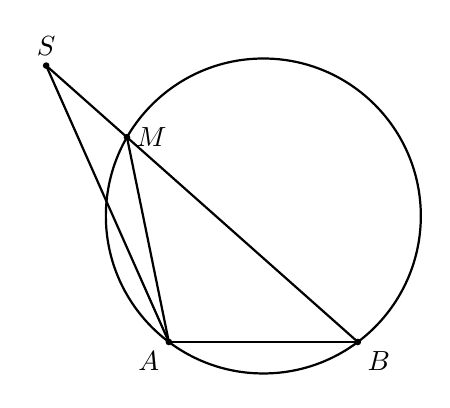
\begin{tikzpicture}[scale=1.0]
  \draw[thick] (0,0) circle (2);
  \coordinate (A) at (-1.2,-1.6);
  \coordinate (B) at (1.2,-1.6);
  \coordinate (M) at (-1.732,1);
  \coordinate (S) at (-2.758,1.91);
  \draw[thick] (S)--(B);
  \draw[thick] (S)--(A);
  \draw[thick] (A)--(B);
  \draw[thick] (A)--(M);
  \fill (A) circle (1.2pt) node[below left] {$A$};
  \fill (B) circle (1.2pt) node[below right] {$B$};
  \fill (M) circle (1.2pt) node[right] {$M$};
  \fill (S) circle (1.2pt) node[above] {$S$};
\end{tikzpicture}
\end{center}
\nopagebreak[4]
\Needspace{5\baselineskip}
设船 $S$ 在圆外，直线 $SB$ 交圆于 $M$（$M$ 在 $S$、$B$ 之间）。在 $\triangle ASM$ 中，$\angle AMB$ 与 $\angle AMS$ 互补，而

\nopagebreak[4]
\[
\angle AMS=180^\circ-\angle ASB-\angle SAM,
\]

\Needspace{5\baselineskip}
于是

\nopagebreak[4]
\[
\angle AMB=\angle ASB+\angle SAM>\angle ASB.
\]

这就是说：圆外任一点到弦的两端的连线的夹角，小于该弦上的圆周角。因此只要 $\angle ASB<\angle AMB$，船就总在暗礁区 $AMB$ 的外面，可以安全进港。

\gkanswer{答案：见解析版}

\end{answer}
\begin{answer}
\gksolhead{4}{}

\textbf{题目}：

\Needspace{5\baselineskip}
（1） 计算：

\nopagebreak[4]
\[
8x^{-\frac13}\sqrt{y^{-\frac13}x^4\sqrt{y^{\frac43}}};
\]

（2） 证明：$\log_a b\cdot\log_b C\cdot\log_c a=1$。

\begin{gktip}
\textbf{源注}：源卷题面第二个对数的真数印作大写 $C$，同题证明行按换底公式以 $\dfrac{\lg b}{\lg a}\cdot\dfrac{\lg c}{\lg b}\cdot\dfrac{\lg a}{\lg c}$ 复算、全用小写；记号大小写不一致系源卷排印，题面照录。
\end{gktip}

\Needspace{5\baselineskip}
（3） 证明：

\nopagebreak[4]
\[
\frac{\operatorname{Sin}(\alpha+\beta)-2\operatorname{Sin}\alpha\operatorname{Cos}\beta}
{2\operatorname{Sin}\alpha\operatorname{Sin}\beta+\operatorname{Cos}(\alpha+\beta)}
=\operatorname{tg}(\beta-\alpha).
\]

（4） 计算：在等比数列里，已知 $a_1=2$，$S_3=26$，求 $q$。

\Needspace{4\baselineskip}
\textbf{解析}

\gksubpart{（1）}

\Needspace{5\baselineskip}
先把内层根式化为分数指数幂：$\sqrt{y^{\frac43}}=\left(y^{\frac43}\right)^{\frac12}=y^{\frac23}$，于是

\nopagebreak[4]
\[
\begin{aligned}
8x^{-\frac13}\sqrt{y^{-\frac13}x^4\sqrt{y^{\frac43}}}
&=8x^{-\frac13}\left[y^{-\frac13}x^4\left(y^{\frac43}\right)^{\frac12}\right]^{\frac12}\\
&=8x^{-\frac13}\left(x^4y^{\frac13}\right)^{\frac12}\\
&=8x^{\frac53}y^{\frac16}
=8x\sqrt[6]{x^4y}.
\end{aligned}
\]

\gksubpart{（2）}

\Needspace{5\baselineskip}
设 $a\text{、}b\text{、}c$ 均为大于 $0$ 且不等于 $1$ 的数。由对数换底公式，

\nopagebreak[4]
\[
\log_a b=\frac{\lg b}{\lg a},
\qquad
\log_b c=\frac{\lg c}{\lg b},
\qquad
\log_c a=\frac{\lg a}{\lg c}.
\]

\Needspace{5\baselineskip}
三式相乘，分子分母依次约去：

\nopagebreak[4]
\[
\log_a b\cdot\log_b c\cdot\log_c a
=\frac{\lg b}{\lg a}\cdot\frac{\lg c}{\lg b}\cdot\frac{\lg a}{\lg c}
=1.
\]

\begin{gktip}
\textbf{源注复核}：源卷题面把第二个真数印作大写 $C$，同题证明行全部用小写；两处记号指同一对象，按同一恒等式处理。
\end{gktip}

\gksubpart{（3）}

\nopagebreak[4]
\[
\begin{aligned}
\text{\text{左边}}
&=\frac{\sin\alpha\cos\beta+\cos\alpha\sin\beta-2\sin\alpha\cos\beta}
{2\sin\alpha\sin\beta+\cos\alpha\cos\beta-\sin\alpha\sin\beta}\\
&=\frac{\cos\alpha\sin\beta-\sin\alpha\cos\beta}
{\cos\alpha\cos\beta+\sin\alpha\sin\beta}\\
&=\frac{\sin(\beta-\alpha)}{\cos(\beta-\alpha)}
=\tan(\beta-\alpha)
=\text{\text{右边}}.
\end{aligned}
\]

恒等式得证。

\gksubpart{（4）}

\Needspace{5\baselineskip}
$a_1=2$，$S_3=26$。由等比数列前 $n$ 项和公式（$q\ne1$），

\nopagebreak[4]
\[
26=\frac{2(1-q^3)}{1-q}.
\]

\Needspace{5\baselineskip}
两边除以 $2$ 并用 $1-q^3=(1-q)(1+q+q^2)$，得

\nopagebreak[4]
\[
1+q+q^2=13,
\qquad
q^2+q-12=0,
\qquad
(q+4)(q-3)=0.
\]

所以 $q_1=-4$，$q_2=3$。验证：$q=-4$ 时 $2-8+32=26$；$q=3$ 时 $2+6+18=26$，均符合。

\gkanswer{答案（1）：$8x^{\frac53}y^{\frac16}$（即 $8x\sqrt[6]{x^4y}$）。}

\gkanswer{答案（2）：见解析版}

\gkanswer{答案（3）：见解析版}

\gkanswer{答案（4）：$q_1=-4$，$q_2=3$。}

\end{answer}
\begin{answer}
\gksolhead{5}{}

\textbf{题目}：

修建水库时，欲测两山腰上 $A\text{、}B$ 两点间的距离，在某处选与 $A\text{、}B$ 在同一平面内 $C\text{、}D$ 两点，测得 $CD=200$ 米，$\angle ACD=105^\circ$，$\angle BCD=15^\circ$，$\angle BDC=120^\circ$，$\angle ADC=30^\circ$，试求 $AB$。

\begin{gktip}
原源 PDF 第 3 页附有四边形 $ABCD$ 与基线 $CD$ 的示意图（标注 $105^\circ$、$15^\circ$、$30^\circ$、$120^\circ$ 与 $200$）；LaTeX 版按源图重绘。
\end{gktip}
\nopagebreak[4]
\begin{center}% 1977 年吉林卷第 5 题：测距示意——四边形 ABCD，
% 基线 CD=200，C 处标 105°、15°，D 处标 30°、120°（按源卷第 3 页布局：A、B 在上）
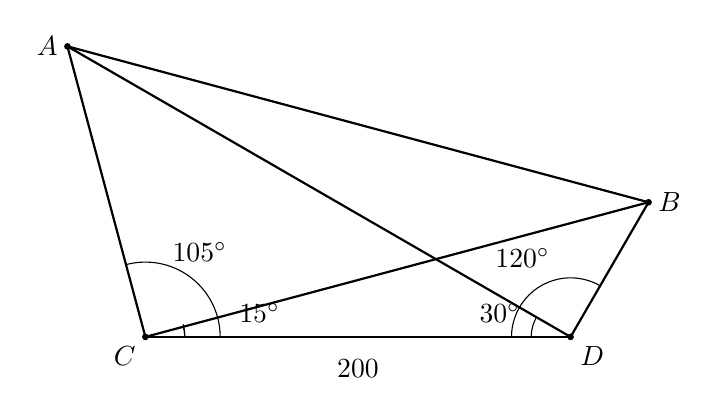
\begin{tikzpicture}[scale=1.0]
  \coordinate (C) at (0,0);
  \coordinate (D) at (5.4,0);
  \coordinate (A) at (-0.99,3.69);
  \coordinate (B) at (6.39,1.71);
  \draw[thick] (A)--(B);
  \draw[thick] (A)--(C);
  \draw[thick] (A)--(D);
  \draw[thick] (B)--(C);
  \draw[thick] (B)--(D);
  \draw[thick] (C)--(D);
  \draw (0.95,0) arc[start angle=0,end angle=105,radius=0.95];
  \draw (0.5,0) arc[start angle=0,end angle=15,radius=0.5];
  \draw (0.5,0) arc[start angle=0,end angle=15,radius=0.62];
  \draw ([shift=(180:0.5)]D) arc[start angle=180,end angle=150,radius=0.5];
  \draw ([shift=(180:0.75)]D) arc[start angle=180,end angle=60,radius=0.75];
  \fill (A) circle (1.2pt) node[left] {$A$};
  \fill (B) circle (1.2pt) node[right] {$B$};
  \fill (C) circle (1.2pt) node[below left] {$C$};
  \fill (D) circle (1.2pt) node[below right] {$D$};
  \node at (0.69,1.08) {$105^\circ$};
  \node at (1.45,0.30) {$15^\circ$};
  \node at (4.5,0.30) {$30^\circ$};
  \node at (4.79,1.00) {$120^\circ$};
  \node at (2.7,-0.4) {$200$};
\end{tikzpicture}
\end{center}
\nopagebreak[4]
\Needspace{4\baselineskip}
\textbf{解析}

\Needspace{5\baselineskip}
在 $\triangle ACD$ 中，

\nopagebreak[4]
\[
\angle CAD=180^\circ-\angle ACD-\angle ADC
=180^\circ-105^\circ-30^\circ=45^\circ.
\]

\Needspace{5\baselineskip}
由正弦定理，

\nopagebreak[4]
\[
AC=\frac{200\sin30^\circ}{\sin45^\circ}
=\frac{200\cdot\frac12}{\frac{\sqrt2}{2}}
=100\sqrt2\ \text{（\text{米}）}.
\]

\Needspace{5\baselineskip}
在 $\triangle BCD$ 中，

\nopagebreak[4]
\[
\angle CBD=180^\circ-\angle BDC-\angle BCD
=180^\circ-120^\circ-15^\circ=45^\circ.
\]

\Needspace{5\baselineskip}
由正弦定理，

\nopagebreak[4]
\[
BC=\frac{200\sin120^\circ}{\sin45^\circ}
=\frac{200\cdot\frac{\sqrt3}{2}}{\frac{\sqrt2}{2}}
=100\sqrt6\ \text{（\text{米}）}.
\]

\Needspace{5\baselineskip}
在 $\triangle ACB$ 中，

\nopagebreak[4]
\[
\angle ACB=\angle ACD-\angle BCD=105^\circ-15^\circ=90^\circ.
\]

\Needspace{5\baselineskip}
由勾股定理，

\nopagebreak[4]
\[
\begin{aligned}
AB&=\sqrt{AC^2+BC^2}
=\sqrt{(100\sqrt2)^2+(100\sqrt6)^2}\\
&=\sqrt{20000+60000}
=200\sqrt2\ \text{（\text{米}）}.
\end{aligned}
\]
\nopagebreak[4]
\begin{center}% 1977 年吉林卷第 5 题：测距示意——四边形 ABCD，
% 基线 CD=200，C 处标 105°、15°，D 处标 30°、120°（按源卷第 3 页布局：A、B 在上）
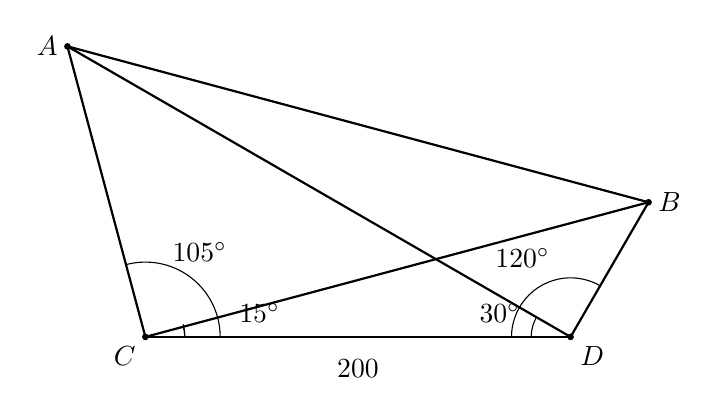
\begin{tikzpicture}[scale=1.0]
  \coordinate (C) at (0,0);
  \coordinate (D) at (5.4,0);
  \coordinate (A) at (-0.99,3.69);
  \coordinate (B) at (6.39,1.71);
  \draw[thick] (A)--(B);
  \draw[thick] (A)--(C);
  \draw[thick] (A)--(D);
  \draw[thick] (B)--(C);
  \draw[thick] (B)--(D);
  \draw[thick] (C)--(D);
  \draw (0.95,0) arc[start angle=0,end angle=105,radius=0.95];
  \draw (0.5,0) arc[start angle=0,end angle=15,radius=0.5];
  \draw (0.5,0) arc[start angle=0,end angle=15,radius=0.62];
  \draw ([shift=(180:0.5)]D) arc[start angle=180,end angle=150,radius=0.5];
  \draw ([shift=(180:0.75)]D) arc[start angle=180,end angle=60,radius=0.75];
  \fill (A) circle (1.2pt) node[left] {$A$};
  \fill (B) circle (1.2pt) node[right] {$B$};
  \fill (C) circle (1.2pt) node[below left] {$C$};
  \fill (D) circle (1.2pt) node[below right] {$D$};
  \node at (0.69,1.08) {$105^\circ$};
  \node at (1.45,0.30) {$15^\circ$};
  \node at (4.5,0.30) {$30^\circ$};
  \node at (4.79,1.00) {$120^\circ$};
  \node at (2.7,-0.4) {$200$};
\end{tikzpicture}
\end{center}
\nopagebreak[4]
即 $AB$ 长为 $200\sqrt2$ 米（约 $282.8$ 米）。

\gkanswer{答案：$AB=200\sqrt2$ 米（约 $282.8$ 米）。}

\end{answer}
\begin{answer}
\gksolhead{6}{}

\textbf{题目}：

已知直线 $4x+3y-12=0$ 和园心在 $(4,7)$ 点的一个园相切，求这园的半径及过园心和切点的直线方程。

\textbf{参考题 1．} 把 $4x^2+9y^2+8x-36y+4=0$ 化成标准方程，并指出它所代表的曲线的长、短半轴、离心率。

\textbf{参考题 2．} 试求下列各式的导数：

（1）$y=3x^2+\sqrt{x}+5$；

（2）$y=\ln(x^{10})+\ln(\ln x)$；

（3）$y=x^x$。

\textbf{参考题 3．} 求微分方程的通解：

（1）$y'=\dfrac{2+y}{3-x}$；

（2）$y''-2y'-3y=0$。

\Needspace{4\baselineskip}
\textbf{解析}

\Needspace{5\baselineskip}
设圆的方程为

\nopagebreak[4]
\[
(x-4)^2+(y-7)^2=R^2.
\]

\Needspace{5\baselineskip}
圆与直线 $4x+3y-12=0$ 相切，故圆心 $(4,7)$ 到直线的距离等于半径：

\nopagebreak[4]
\[
R=\frac{|4\cdot4+3\cdot7-12|}{\sqrt{4^2+3^2}}
=\frac{25}{5}=5.
\]

\Needspace{5\baselineskip}
于是圆的方程为 $(x-4)^2+(y-7)^2=25$。求圆与直线的交点，联立

\nopagebreak[4]
\[
\begin{cases}
(x-4)^2+(y-7)^2=25,\\
4x+3y-12=0.
\end{cases}
\]

\Needspace{5\baselineskip}
把 $y=\dfrac{12-4x}{3}$ 代入圆方程并整理：

\nopagebreak[4]
\[
9(x-4)^2+(4x+9)^2=225,
\]

\nopagebreak[4]
\[
25x^2+225=225,
\qquad
x=0,
\qquad
y=4.
\]

\Needspace{5\baselineskip}
方程组得两组相同的解，表示 $(0,4)$ 是切点。过圆心 $(4,7)$ 与切点 $(0,4)$ 的直线，斜率为 $\dfrac{7-4}{4-0}=\dfrac34$，方程为

\nopagebreak[4]
\[
y-4=\frac34x,
\]

\Needspace{5\baselineskip}
即

\nopagebreak[4]
\[
3x-4y+16=0.
\]

\textbf{参考题 1}

\Needspace{5\baselineskip}
原方程配方：

\nopagebreak[4]
\[
4(x^2+2x+1)+9(y^2-4y+4)-36=0,
\]

\Needspace{5\baselineskip}
即

\nopagebreak[4]
\[
4(x+1)^2+9(y-2)^2=36.
\]

\Needspace{5\baselineskip}
标准方程为

\nopagebreak[4]
\[
\frac{(x+1)^2}{3^2}+\frac{(y-2)^2}{2^2}=1.
\]

\Needspace{5\baselineskip}
它表示以 $(-1,2)$ 为中心的椭圆，长半轴 $a=3$，短半轴 $b=2$。半焦距

\nopagebreak[4]
\[
c=\sqrt{a^2-b^2}=\sqrt{9-4}=\sqrt5,
\]

\Needspace{5\baselineskip}
离心率

\nopagebreak[4]
\[
e=\frac{c}{a}=\frac{\sqrt5}{3}.
\]

\textbf{参考题 2}

（1）

\Needspace{5\baselineskip}
$y=3x^2+\sqrt{x}+5$，

\nopagebreak[4]
\[
y'=6x+\frac{1}{2\sqrt{x}}.
\]

（2）

\Needspace{5\baselineskip}
$y=\ln(x^{10})+\ln(\ln x)$，

\nopagebreak[4]
\[
y'=\frac{10x^9}{x^{10}}+\frac{\dfrac1x}{\ln x}
=\frac{10}{x}+\frac{1}{x\ln x}.
\]

（3）

\Needspace{5\baselineskip}
$y=x^x=\mathrm e^{x\ln x}$，

\nopagebreak[4]
\[
y'=\mathrm e^{x\ln x}(\ln x+1)=x^x(1+\ln x).
\]

\textbf{参考题 3}

（1）

\Needspace{5\baselineskip}
$y'=\dfrac{2+y}{3-x}$ 是可分离变量的方程，写成

\nopagebreak[4]
\[
\frac{dy}{2+y}=\frac{dx}{3-x}.
\]

\Needspace{5\baselineskip}
两边积分，

\nopagebreak[4]
\[
\ln|2+y|=-\ln|3-x|+C_1,
\]

\Needspace{5\baselineskip}
即

\nopagebreak[4]
\[
2+y=\frac{C}{3-x}
\qquad(C=\mathrm e^{C_1}).
\]

\Needspace{5\baselineskip}
所以通解为

\nopagebreak[4]
\[
y=\frac{C}{3-x}-2
\qquad(C\ \text{\text{为任意常数}}).
\]

（2）

\Needspace{5\baselineskip}
$y''-2y'-3y=0$ 是二阶常系数齐次线性方程，其特征方程为

\nopagebreak[4]
\[
\lambda^2-2\lambda-3=0,
\]

\Needspace{5\baselineskip}
根是 $\lambda_1=3$，$\lambda_2=-1$，因此原方程的通解为

\nopagebreak[4]
\[
y=C_1\mathrm e^{3x}+C_2\mathrm e^{-x},
\]

其中 $C_1\text{、}C_2$ 是任意常数。

\gkanswer{答案：圆的半径 $R=5$；切点为 $(0,4)$，过圆心和切点的直线方程为 $3x-4y+16=0$。}

\end{answer}